\section{Adapting to {\sc Boost} Graphs\label{arr_sec:bgl}}
%=======================================

\boost\footnote{See also {\sc Boost}'s homepage at: {\tt www.boost.org}.}
is a collection of portable \CC\
libraries that extend the Standard Template Library ({\sc Stl}). The \boost\
Graph Library (\bgl), which one of the libraries in the collection, offers an
extensive set of generic graph algorithms parameterized through templates.
As our arrangements are embedded as planar graphs, it is only 
natural to extend the underlying data structure with the interface that the 
\bgl\ expects, and gain the ability to perform the operations that the \bgl\
supports, such as shortest-path computation. This section describes how apply
the graph algorithms implemented in the \bgl\ to \ccc{Arrangement_2} instances.

An instance of \ccc{Arrangement_2} is adapted to a \boost\ graph through the
provision of a set of free functions that operate on the arrangement features
and conform with the relevant BGL concepts. Besides the straightforward 
adaptation, which associates a vertex with each \dcel\ vertex and an edge 
with each \dcel\ halfedge, the package also offer a {\em dual} adaptor, which 
associates a graph vertex with each \dcel\ face, such that two vertices are 
connected, iff there is a \dcel\ halfedge that connects the two corresponding
faces. 

\subsection{The Primal Arrangement Representation\label{arr_ssec:bgl_primal}}
%-------------------------------------------------

Arrangement instances are adapted to \boost\ graphs by specializing the
\ccc{boost::graph_traits} template for \ccc{Arrangement_2} instances. The
graph-traits states the graph concepts that the arrangement class models
(see below) and defines the types required by these concepts.

In this specialization the \ccc{Arrangement_2} vertices correspond to the
graph vertices, where two vertices are adjacent if there is at least one
halfedge connecting them. More precisely, \ccc{Arrangement_2::Vertex_handle}
is the graph-vertex type, while \ccc{Arrangement_2::Halfedge_handle} is the
graph-edge type. As halfedges are directed, we consider the graph to be
directed as well. Moreover, as several interior-disjoint $x$-monotone curves
(say circular arcs) may share two common endpoints, inducing an arrangement
with two vertices that are connected with several edges, we allow parallel
edges in our \boost\ graph.

Given an \ccc{Arrangement_2} instance, we can efficiently traverse its
vertices and halfedges. Thus, the arrangement graph is a model of the concepts
\ccc{VertexListGraph} and \ccc{EdgeListGraph} introduced by the \bgl.
At the same time, we use an iterator adapter of the circulator over the
halfedges incident to a vertex (\ccc{Halfedge_around_vertex_circulator} --- see
Section~\ref{arr_sssec:tr_vertex}), so it is possible to go over the ingoing
and outgoing edges of a vertex in linear time. Thus, our arrangement graph
is a model of the concept \ccc{BidirectionalGraph} (this concept refines
\ccc{IncidenceGraph}, which requires only the traversal of outgoing edges).

It is important to notice that the vertex descriptors we use are
\ccc{Vertex_handle} objects and {\em not} vertex indices. However, in order
to gain more efficiency in most \bgl\ algorithm, it is better to have them
indexed $0, 1, \ldots, (n-1)$, where $n$ is the number of vertices. We
therefore introduce the \ccc{Arr_vertex_index_map<Arrangement>} class-template,
which maintains a mapping of vertex handles to indices, as required by the
\bgl. An instance of this class must be attached to a valid arrangement
vertex when it is created. It uses the notification mechanism (see
Section~\ref{arr_sec:notif}) to automatically maintain the mapping of vertices
to indices, even when new vertices are inserted into the arrangement or
existing vertices are removed.

In most algorithm provided by the \bgl, the output is given by
{\em property maps}, such that each map entry corresponds to a vertex.
For example, when we compute the shortest paths from a given source vertex
$s$ to all other vertices we can obtain a map of distances and a map of
predecessors --- namely for each $v$ vertex we have its distance from $s$
and a descriptor of the vertex that precedes $v$ in the shortest path from $s$.
If the vertex descriptors are simply indices, boost supplies tools to
easily represent property maps using vectors.
\ccc{Arr_vertex_index_map<Arrangement>} class allows create such
indices, and together with \ccc{boost::vector_property_map<Type,
  IndexMap>} allows for
an efficient mapping of \ccc{Vertex_handle} objects to
properties of type \ccc{Type}. Note however that unlike the
\ccc{Arr_vertex_index_map} class, the vertex property-map class is not
kept synchronized with the number of vertices in the arrangement, so it
should not be reused in calls to \bgl\ functions in case the arrangement
is modified in between these calls.

\begin{figure}[t]
\begin{ccTexOnly}
  \begin{center}
  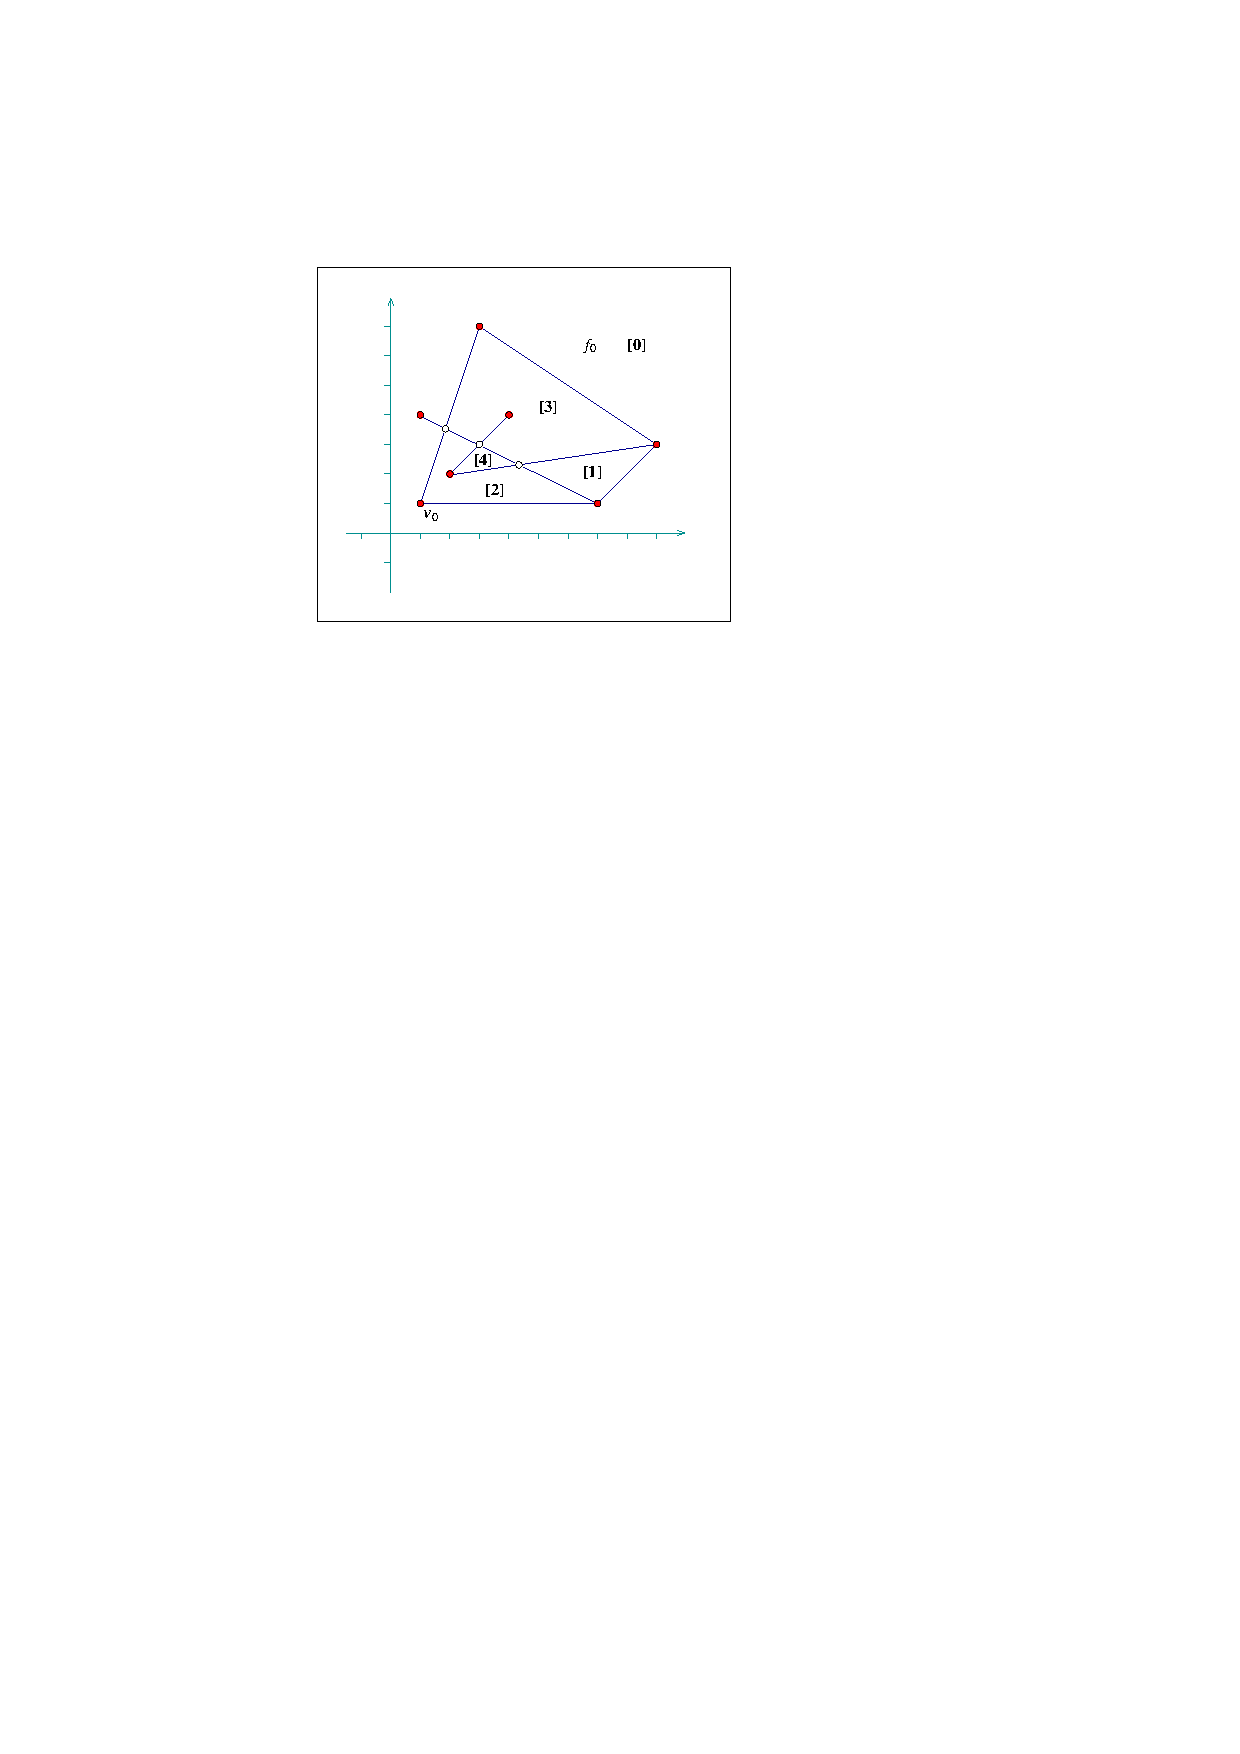
\includegraphics{Arrangement_on_surface_2/fig/ex_bgl}
  \end{center}
\end{ccTexOnly}
\begin{ccHtmlOnly}
  <p><center>
  <img src="./fig/ex_bgl.gif" border=0 alt="Example BGL">
  </center>
\end{ccHtmlOnly}
\caption{An arrangement of 7 line segments, as constructed by
\ccc{bgl_primal_adapter.cpp} and \ccc{bgl_dual_adapter.cpp}.
The breadth-first visit times for the arrangement faces, starting
from the unbounded face $f_0$, are shown is brackets.}
\label{arr_fig:ex_bgl}
\end{figure}

In the following example we construct an arrangement of 7 line segments,
as shown in Figure~\ref{arr_fig:ex_bgl},
then use Dijkstra's shortest-paths algorithm from the \bgl\ to compute
the graph distance of all vertices from the leftmost vertex in the
arrangement $v_0$. Note the usage of the \ccc{Arr_vertex_index_map} and
the \ccc{boost::vector_property_map<Type, IndexMap>} classes. The
latter one, instantiated by the type \ccc{double} is used to map
vertices to their distances from $v_0$.

\ccIncludeExampleCode{Arrangement_on_surface_2/bgl_primal_adapter.cpp}

\subsection{The Dual Arrangement Representation\label{arr_ssec:bgl_dual}}
%-----------------------------------------------

It is possible to give a dual graph representation for an arrangement instance,
such that each arrangement face corresponds to a graph vertex and two vertices
are adjacent iff the corresponding faces share a common edge on their
boundaries. This is done by specializing the
\ccc{boost::graph_traits} template for \ccc{Dual<Arrangement_2>} instances,
where \ccc{Dual<Arrangement_2>} is a template specialization that gives a
dual interpretation to an arrangement instance.

In dual representation, \ccc{Arrangement_2::Face_handle}
is the graph-vertex type, while \ccc{Arrangement_2::Halfedge_handle} is the
graph-edge type. We treat the graph edges as directed, such that a halfedge
\ccc{e} is directed from $f_1$, which is its incident face, to $f_2$, which
is the incident face of its twin halfedge. As two arrangement faces may
share more than a single edge on their boundary, we allow parallel
edges in our \boost\ graph. As is the case in the primal graph, the dual
arrangement graph is also a model of the concepts \ccc{VertexListGraph},
\ccc{EdgeListGraph} and \ccc{BidirectionalGraph} (thus also of 
\ccc{IncidenceGraph}).

Since we use \ccc{Face_handle} objects as the vertex descriptors, we define
the \ccc{Arr_face_index_map<Arrangement>} class-template, which maintains an
efficient mapping of face handles to indices.
Like vertices, \ccc{boost::vector_property_map<Type, IndexMap>} can be
used for associating arbitrary data with the arrangement faces.

In the following example we construct the same arrangement as in
example \ccc{bgl_primal_adapter.cpp} (see Figure~\ref{arr_fig:ex_bgl}),
and perform breadth-first search on the graph faces, starting from the
unbounded face. We extend the \dcel\ faces
with an unsigned integer, marking the discover time of the face
using \boost\ visitors and a property-map class that directly accesses
the extended data of the faces:

\ccIncludeExampleCode{Arrangement_on_surface_2/bgl_dual_adapter.cpp}
